\chapter{Inquadramento dello stage}
\label{cap:inquadramento-stage}

\intro{Lo stage, come anche questo documento, si divide in due parti. La prima parte si concentra sullo studio dei \emph{JWT}, metodi di firma e metodi di crittografia. La seconda parte riguarda invece l'implementazione di un \emph{ChatBot} per la piattaforma di messaggistica Microsoft Teams, utilizzando \emph{JWT} firmati e crittografati}\\

\section{Introduzione alla ricerca}
Il processo dell'autenticazione è l'atto di verificare le credenziali dell'utente in termini di correttezza o tempo\footcite{site:token-cookie-auth}.

Per correttezza si intende che le credenziali siano valide e che l'utente sia chi dice di essere.
Al momento dell'accesso, un token di autenticazione\footnote{In questo contesto, per token di autenticazione si intende una qualsiasi forma di credeziale di autentiazione.} viene assegnato all'utente.
Questo token viene utilizzato per verificare l'identità dell'utente in ogni richiesta successiva.

Per tempo, invece, si intende che l'utente abbia accesso al sistema per un periodo di tempo limitato.
Questo periodo di tempo è definito dal tempo di scadenza del token.
Quando il token scade, l'utente deve autenticarsi nuovamente per ottenere un nuovo token.

L'autenticazione è un processo fondamentale per la sicurezza di un'applicazione.
Essa, infatti, permette di verificare che l'utente sia chi sostiene di essere, dando ad ogni utente un'identità univoca che protegge i dati dell'utente stesso negando l'accesso a soggetti non autorizzati.

Esistono principalmente due metodi di autenticazione: l'autenticazione basata su \emph{\gls{web cookie}} e l'autenticazione basata su token.

\subsection{Autenticazione basata su web cookie}
Un web cookie, o più semplicemente cookie, è un piccolo blocco di dati creato da un server web e inviato all'utente\footcite{site:cookie-wikipedia}.
Questi dati sono spesso essenziali per il funzionamento di un sito web, in quanto permettono di memorizzare, oltre alla sessione dell'utente, informazioni salvate dall'utente stesso, come le preferenze sull'aspetto grafico o gli articoli aggiunti al carrello.

L'utilizzo dei cookie per l'autenticazione è considerato l'approccio classico ed è spesso indicato come autenticazione basata su sessione. 
Questo perché il server li genera con un ID di sessione che memorizza nel proprio database e invia al client\footnote{Il client fa parte dell'architettura client-server ed è l'entità che richiede risorse o servizi da un server. Nel contesto delle applicazioni web, il client è tipicamente rappresentato dal browser web o da un'applicazione che l'utente utilizza per interagire con il server. Il client invia richieste al server e riceve risposte che possono includere dati, pagine web, file o altri contenuti.}.
Il client, ogni volta che fa una richiesta al server, invia il cookie con l'ID di sessione che il server utilizza per identificare l'utente, verificandone la validità.

L'autenticazione basata su cookie è considerata con stato (dall'inglese \emph{stateful}) in quanto sia il client che il server devono mantenere lo stato della sessione. \\

\noindent Il procedimento completo di autenticazione basata su cookie, illustrato in figura \ref{fig:auth-cookie-based}, è il seguente:
\begin{enumerate}
	\item L'utente che vuole accedere alla risorsa protetta inserisce le proprie credenziali.
	\item Il server verifica le credenziali e, se corrette, crea un cookie con un ID di sessione univoco.
	\item Il cookie viene inviato al client, il cui browser memorizza in modo automatico.
	\item Il client, ogni volta che fa una richiesta al server, invia il cookie con l'ID di sessione.
	\item Una volta verificato dal server, all'utente viene permesso l'accesso alla risorsa protetta.
	\item In caso di scadenza del cookie, l'utente deve autenticarsi nuovamente per ottenerne uno nuovo.
	\item Quando viene effettuato il logout, il cookie viene cancellato dal client e invalidato dal server.
\end{enumerate}

\begin{figure}[!ht] 
    \centering 
    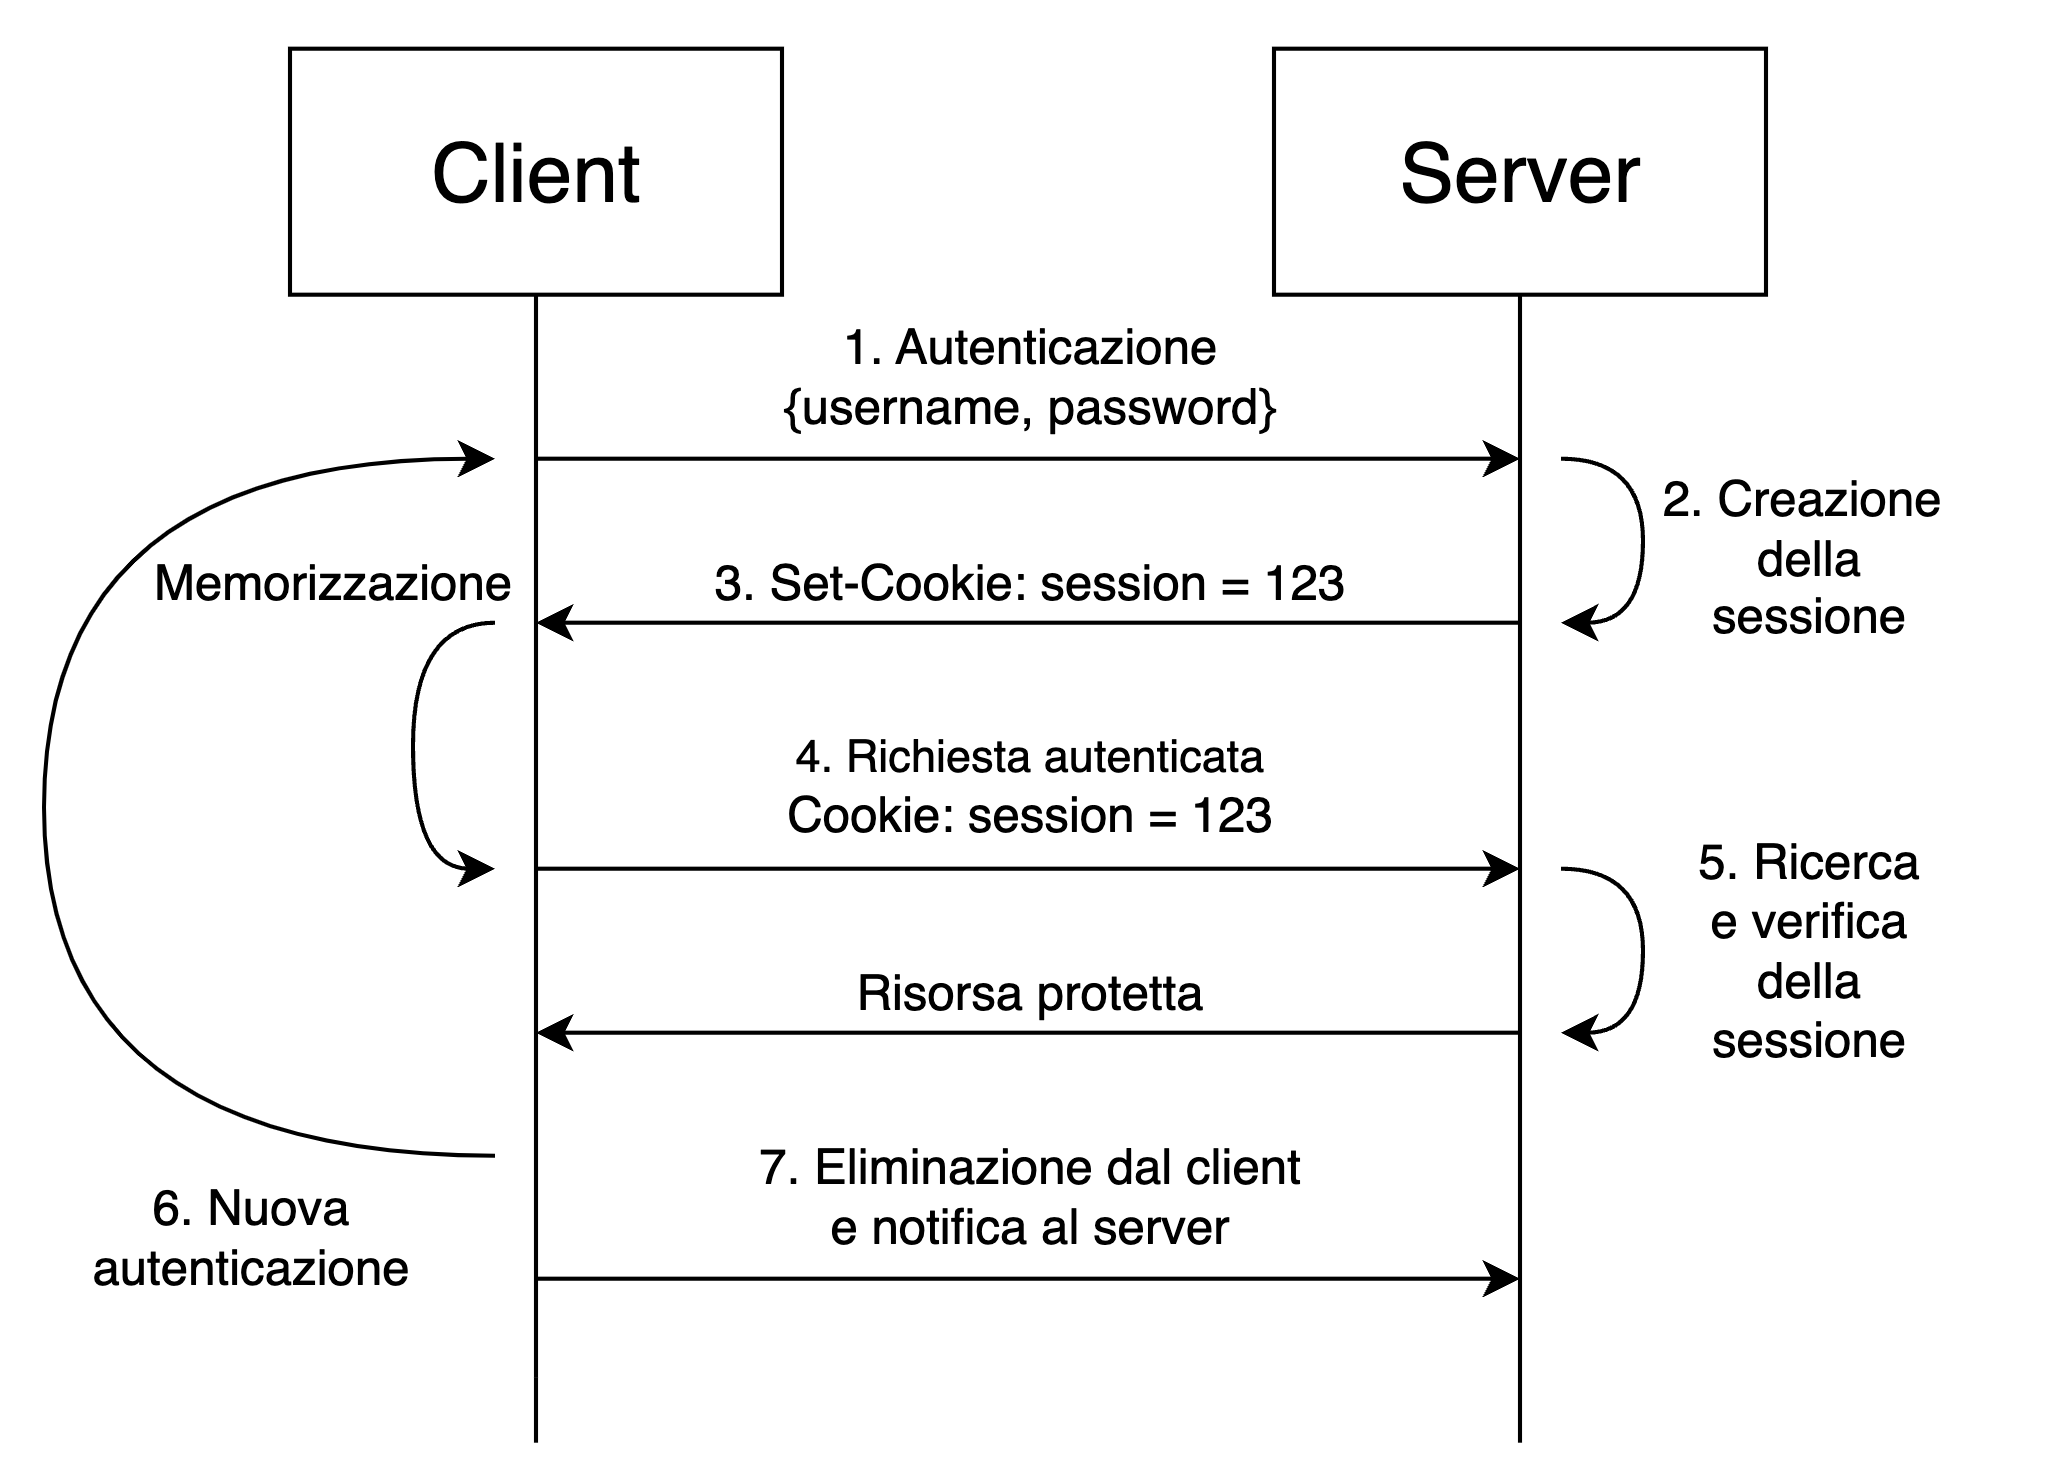
\includegraphics[width=0.9\columnwidth]{descrizione-stage/auth-cookie-based} 
    \caption{Processo di autenticazione basato su cookie}
	\label{fig:auth-cookie-based}
\end{figure}

\noindent L'utilizzo di cookie per l'autenticazione ha molti vantaggi.
Il principale è che sono supportati da tutti i browser e sono facili da implementare, in quanto è il browser stesso a gestirne la memorizzazione e l'invio.
I cookie inoltre necessitano di poca memoria e possono essere utilizzati anche per i \emph{sottodomini} di un sito web.

Tuttavia, l'autenticazione basata su cookie ha anche dei limiti.
Infatti, essi sono vulnerabili ad attacchi di tipo \emph{Cross-Site Scripting (XSS)} e \emph{Cross-Site Request Forgery (CSRF)} e non sono adatti per le architetture senza stato (dall'inglese \emph{stateless}), come alcuni tipi di \emph{\gls{API}}.
Inoltre, i cookie non sono facilmente scalabili e non sono adatti per le applicazioni distribuite, in quanto dovrebbero essere memorizzati in un \emph{database} condiviso che potrebbe aumentare la complessità dell'applicazione.

\subsection{Autenticazione basata su token}
Un metodo di autenticazione alternativo all'utilizzo dei cookie è l'autenticazione basata su token.
Questo metodo è diventato molto popolare negli ultimi anni grazie all'aumento delle applicazioni web single page, al maggiore utilizzo di \emph{\gls{API RESTful}} e dalla diffusione di dispositivi \emph{\gls{IoT}}.

Un token è un oggetto simbolico rilasciato da un'autorità fidata\footcite{site:token-based-authentication-cloudflare}, ovvero il server, che permette all'utente di accedere a una risorsa protetta.
Diversamente dai cookie, i token sono \emph{stateless}, dunque non è necessaria la memorizzazione di alcuna informazione sul server.
Ciò è possibile perché ogni token contiene tutte le informazioni necessarie per la verifica dell'identità dell'utente e per l'accesso alla risorsa protetta. \\

\noindent Analogamente ai cookie, l'autenticazione basata su token viene effettuata nel seguente modo, come illustrato in figura \ref{fig:auth-token-based}:
\begin{enumerate}
	\item L'utente che vuole accedere alla risorsa protetta inserisce le proprie credenziali.
	\item Il server verifica le credenziali e, se corrette, genera un token con tutte le informazioni necessarie per l'accesso alla risorsa protetta.
	\item Il token viene inviato al client, il quale lo memorizza in modo sicuro.
	\item A questo punto, quando il client ha bisogno di accedere a una risorsa prottetta, include il token nella richiesta.
	\item Il server verifica la sua validità e consente l'accesso alla risorsa richiesta. 
	\item In caso di scadenza, l'utente deve autenticarsi nuovamente per ottenere un nuovo token.
	\item Quando viene effettuato il logout, il token viene cancellato dal client. Il server, invece, essendo senza stato, non ha bisogno di effettuare ulteriori operazioni.
\end{enumerate}

\begin{figure}[!ht] 
	\centering 
	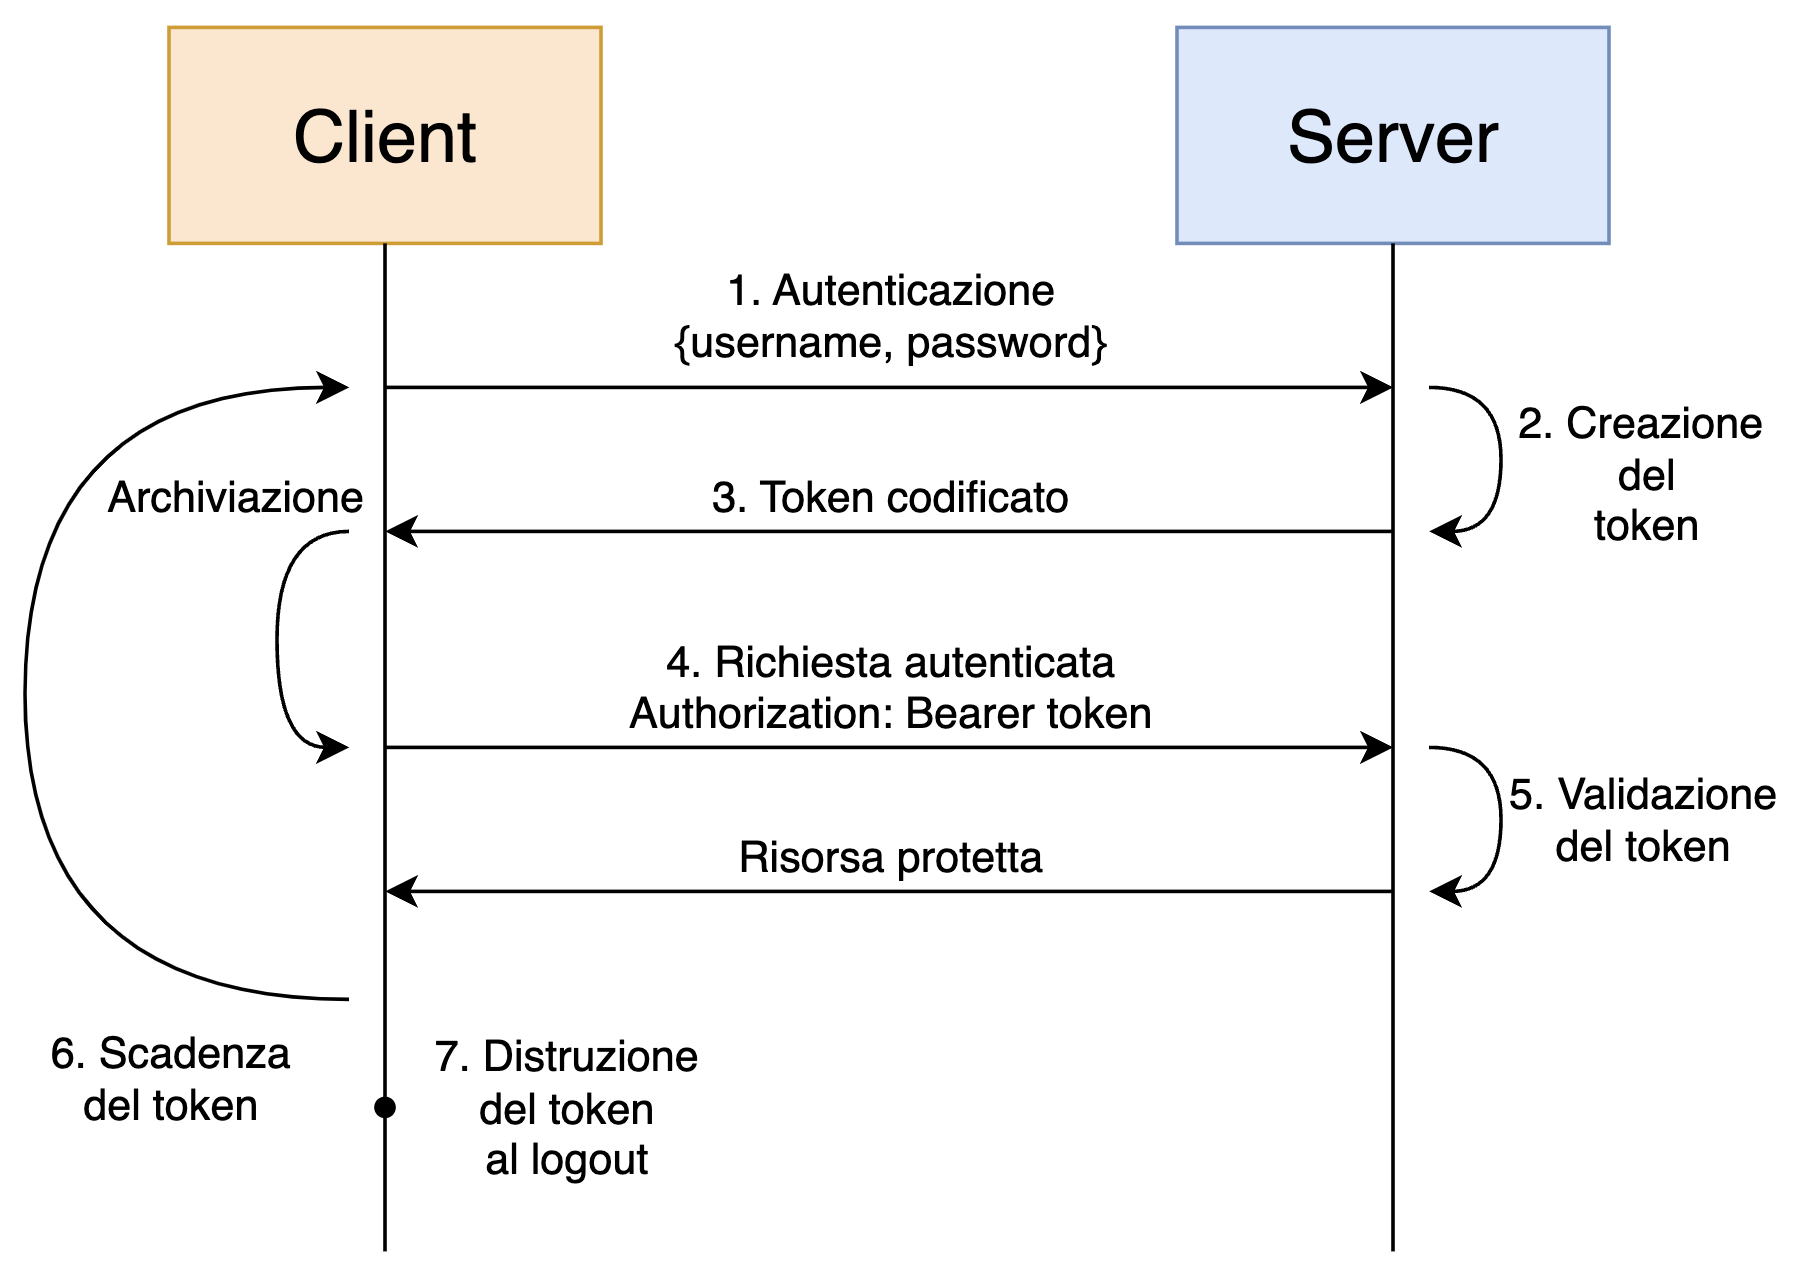
\includegraphics[width=0.9\columnwidth]{descrizione-stage/auth-token-based} 
	\caption{Processo di autenticazione basato su token}
	\label{fig:auth-token-based}
\end{figure}

\noindent L'utilizzo di questo metodo di autenticazione permette, dal lato server, di velocizzarne il processo, poiché non è necessaria nessuna verifica nel database.
Inoltre, la presenza di dati addizionali all'interno del token, come il livello dei permessi dell'utente, consente di semplificare ulteriormente il processo.
D'altro canto, questi campi addizionali aumentano notevolmente le dimensioni, rendendo la trasmissione e l'archiviazione più onerose.

Tuttavia, il più grande vantaggio dell'autenticazione basata su token è la possibilità di essere utilizzata anche per applicazioni mobili e \emph{API} che non si interfacciano con un browser.
I cookie, infatti, non si interfacciano correttamente con applicazioni native per dispositivi mobili, mentre i token possono essere facilmente integrati in qualsiasi applicazione con le stesse \emph{API}, se scritti correttamente.
In aggiunta, sono anche facilmente implementabili in applicazioni distribuite, come quelle per dispositivi \emph{IoT}.\\

\noindent Questo documento si concentra sull'autenticazione basata su token, in particolare su quelli di tipo \emph{JSON Web Token (JWT)}.


\section{Introduzione all'implementazione}
Uno dei vantaggi dell'utilizzo di metodi \emph{stateless} è la possibilità di integrarli facilmente in qualsiasi applicazione, indipendentemente dalla tecnologia utilizzata.
L'impossibilità di utilizzare i cookie senza l'ausilio di un browser rende i token la scelta migliore per applicazioni che utilizzano \emph{API RESTful}.

Per completare questo studio, è stato richiesto di implementare un \emph{ChatBot} in \emph{C\#} per la piattaforma di messaggistica Microsoft Teams utilizzando le \emph{API} di Microsoft Graph e token firmati e crittografati per garantire la sicurezza e la riservatezza di tutti i dati scambiati.

\subsection{Microsoft Teams}

\begin{figure}[!ht] 
	\centering 
	
\includegraphics[width=0.3\columnwidth]{descrizione-stage/logo-teams} 
	\caption{Logo di Microsoft Teams}
\end{figure}

Microsoft Teams\footcite{site:microsoft-teams} è una piattaforma di messaggistica e collaborazione offerta da Microsoft.
Essa consente a organizzazioni, team e singoli utenti di comunicare e collaborare con colleghi e clienti in tempo reale tramite chat, videoconferenze e chiamate.
Il \emph{ChatBot} implementato su questa piattaforma consentirà ai clienti di Prorob S.r.l di interagire con i servizi di Quindi Production Copilot in un modo più semplice e veloce.

\subsection{Microsoft Graph}

\begin{figure}[!ht] 
	\centering 
	
\includegraphics[width=0.3\columnwidth]{descrizione-stage/logo-graph} 
	\caption{Logo di Microsoft Graph}
\end{figure}

Microsoft Graph\footcite{site:microsoft-graph} è una piattaforma di sviluppo che unifica le \emph{API} di Microsoft 365 e Azure, permettendo alle applicazioni sviluppate da terze parti di interagire con i dati memorizzati nei vari servizi di Microsoft.
Utilizzando le \emph{API} di Microsoft Graph, il \emph{ChatBot} può interagire con con la chat di Teams, inviando messaggi e ricevendo notifiche.

\section{Obiettivi}
Prima dell'inizio dello stage Prorob S.r.l ha definito un piano di lavoro con gli obiettivi da raggiungere durante le 300-320 ore di stage. \\

\noindent Gli obiettivi principali prevedevano:
\begin{itemize}
	\item Studio dei \emph{JSON Web Token} e dei loro metodi di firma e di crittografia.
	\item Implementazione di una tecnologia generatrice di token \emph{API} firmati con certificati creati da chiavi ellittiche ed autenticati con metodologia \emph{HMAC}.
	\item Contribuire attivamente all'organizzazione e all'avanzamento delle attività in team.
\end{itemize}

Tuttavia, durante le settimane di stage, gli obiettivi iniziali sono stati rivisti in base alle esigenze emerse. Questo ha portato alla rimozione del un obiettivo e alla definizione di uno nuovo.
Infatti è stata rimossa l'implementazione della tecnologia generatrice di token \emph{API} firmati ed è stata sostituita con l'implementazione di un \emph{ChatBot} per la piattaforma di Microsoft Teams utilizzando i \emph{JWT} e algorithmi di firma e crittografia. \\

\noindent Gli obiettivi finali, dunque, sono stati:
\begin{itemize}
	\item Studio dei \emph{JSON Web Token} e dei loro metodi di firma e di crittografia.
	\item Implementazione di un \emph{ChatBot} per la piattaforma di messaggistica Microsoft Teams utilizzando i \emph{JWT} e algoritmi di firma e crittografia.
	\item Contribuire attivamente all'organizzazione e all'avanzamento delle attività in team.
\end{itemize}